\documentclass{scrartcl}
\usepackage{mm_ws15}
\usetikzlibrary{patterns}

\newcommand{\sheetTitle}{Blatt 12, Abgabe 26.1.2016}

\newcommand{\DD}{\mathcal{D}}
\begin{document}
\maketitle

%%%%%%%%%%%%%%%%%%%%%%%%%%%%%%%%%%%%%%%%%%%%%%%%%%%%%%%%%%%%%%%%%%%%%%%%%%%%%%%%
\section{Gradient \points{6}}
\label{sec:gradient}

\begin{subex}
  \item\points{2} An welchen Punkten ist der Gradient von $\mat V(\mat r) = x^3 + y^3 + z^3 - 3xyz$ senkrecht zur $x$-Achse?
  Wo ist er gleich 0?
  \item\points{2} Berechnen Sie $\nabla f(r)$ für $r = \sqrt{x^2 + y^2 + z^2}$ und eine einmal stetig differenzierbare Funktion $f$.
  \item\points{2} Gegeben Sei das Potential $\phi(x, y, z) = \frac{1}{r}$ für $r = \sqrt{x^2 + y^2 + z^2}$. In welchen Raumpunkten $\mat r \in \RR^3$ gilt $\Vert \nabla \phi (\mat r) \Vert = 1$?
\end{subex}

%%%%%%%%%%%%%%%%%%%%%%%%%%%%%%%%%%%%%%%%%%%%%%%%%%%%%%%%%%%%%%%%%%%%%%%%%%%%%%%%
\section{Gradientenfelder I \points{10}}
\label{sec:gradientenfelder1}

In der Vorlesung haben Sie den Begriff des \emph{Gradientenfeldes} kennengelernt.
Ein Gradientenfeld im $\RR^N$ ist eine Funktion $\mat V\colon \DD(\mat V) \to \RR^N$, für die es ein \emph{Potential} $\phi\colon \DD(\mat V) \to \RR$ gibt, sodass
\[
  \label{eq:potential}
  \tag{$\ast$}
  \mat V(\mat r) = \nabla \phi(\mat r).
\]
Hierbei bezeichnen $\DD(\mat V) \subset \RR^N$ den Definitionsbereich der Funktion $V$.
Eine notwendige Bedingung, dass $\mat V$ ein Gradientenfeld ist sind die sogenannten Integrabilitätsbedingungen (Formel (5.18) im Skript für $N = 3$)
\[
  \pderiv[V_i]{x_j} = \pderiv[V_j]{x_i} \quad (i,j=1,\ldots,N).
\]  
\begin{subex}
  \item\points{1} Zeigen Sie, dass jedes Gradientenfeld die Integrabilitätsbedingungen erfüllt.
  \item\points{4} Berechnen Sie die Vektorfelder der folgenden Potentiale
  \[
    \phi_1(x,y,z) = x^2 y + z \cos xy, \quad\quad \phi_2 (x,y,z) = r^n \mbox{ mit } r = \sqrt{x^2 + y^2 + z^2} 
  \]
  \item\points{5} Berechnen Sie jeweils ein Potential für die nachfolgenden Gradientenfelder
  \begin{align*}
    \mat V_1(x,y,z) &= \left( x^2 + y^2 + z^2 \right)^{-\frac{3}{2}} \, \colvec{x \\ y \\ z} \\
    \mat V_2(x,y) &= \colvec{6x \cos y \\ -3x^2 \sin y + 2y}.
  \end{align*}
\end{subex}
\begin{remark}{Hinweis}
  Zu c): Schreiben Sie Gleichung~\eqref{eq:potential} komponentenweise auf und lösen Sie nach $\phi$ auf, indem Sie über die Variable integrieren, nach der $\phi$ abgeleitet wird.
  Beachten Sie, dass Integration über eine Variable eine Konstante erzeugt, die u.U. von den anderen Variablen abhängt.
\end{remark}

%%%%%%%%%%%%%%%%%%%%%%%%%%%%%%%%%%%%%%%%%%%%%%%%%%%%%%%%%%%%%%%%%%%%%%%%%%%%%%%%
\section{Gradientenfelder II \points{14}}
\label{sec:gradientenfelder2}

Als nächstes betrachten wir eine wichtige Eigenschaft von Gradientenfeldern.
Ein Vektorfeld $\mat V\colon \DD(\mat V) \to \RR^N$ heißt konservativ, wenn das Wegintegral $\int_\gamma \mat V(\mat r) \cdot \dd \mat r$ nur vom Anfangs- und Endpunkt von $\gamma$ abhängt.

Genauer: Betrachte Wege $\gamma_i\colon [0,1] \to \DD(\mat V)$ ($i=1,2$), die ganz in $\DD(\mat V)$ verlaufen und die gleichen Anfangs-/Endpunkte haben: 
\[
  \gamma_1(0) = \gamma_2(0) \mbox{ und } \gamma_1(1) = \gamma_2(1).
\]
Dann gilt
\[
  \int_{\gamma_1} \mat V(\mat r) \cdot \dd \mat r = \int_{\gamma_2} \mat V(\mat r) \cdot \dd \mat r.
\]
Ein Vektorfeld ist genau dann konservativ, wenn es ein Gradientenfeld ist.
\begin{subex}
  \item\points{6} Entscheiden Sie ob die Vektorfelder vom letzten Übungsblatt, Aufgabe 4 konservativ sind:
  \[
    \mat F_1(x, y) = \colvec{4x + xy \\ \frac{x^2}{2}} \quad \mbox{und} \quad \mat F_2 (x, y) = \colvec{4x + xy \\ x^2}
  \]
  Geben Sie auch entweder ein Potential an oder weisen Sie nach, dass die Integrabilitätsbedingungen nicht erfüllt sind.
  \item\points{2} Zeigen Sie, dass das Vektorfeld
  \[
    \mat V(x,y) = \left(- \frac{y}{x^2 + y^2}, \frac{x}{x^2 + y^2} \right)^T
  \]
  die Integrabilitätsbedingungen erfüllt.
  \item\points{6} Berechnen Sie das Wegintegral über $\mat V$ über den oberen und unteren Halbkreisbogen von $(1,0)$ nach $(-1,0)$ mit Radius $1$(siehe Skizze).
\end{subex}
\begin{center}
  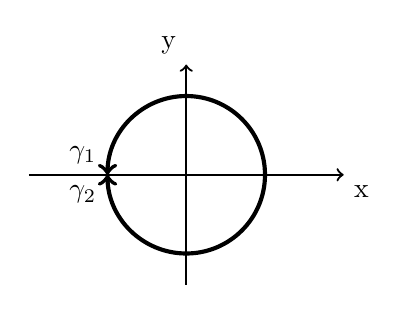
\begin{tikzpicture}[
    curve/.style={->,line width=1.5pt}
  ]
    \draw[thick, ->] (-2,0) -- (2,0) node[anchor = north west] {x};
    \draw[thick, ->] (0,-1.4) -- (0,1.4) node[anchor = south east] {y};
    \draw[curve] (1,0) arc (0:180:1) node [anchor=south east] {$\gamma_1$};
    \draw[curve] (1,0) arc (0:-180:1) node [anchor=north east] {$\gamma_2$};
  \end{tikzpicture}
\end{center}


\begin{remark}{Bemerkung}
  Die Umkehrung: $\mat V$ erfüllt Integrabilitätsbedinungen $\implies$ $\mat V$ Gradientenfeld gilt nur falls $\mat V$ einen einfach zusammenhängenden Definitionsbereich $\DD(\mat V)$ hat.
  Eine Menge $A \subset \RR^N$ heißt dabei \emph{einfach zusammenhängend}, wenn man jeden geschlossenen Weg (d.h. Anfangs- = Endpunkt) auf einen Punkt stetig zusammenziehen kann ohne $A$ dabei zu verlassen. Als Beispiel dienen die folgende Mengen im $\RR^2$:

  \begin{center}
    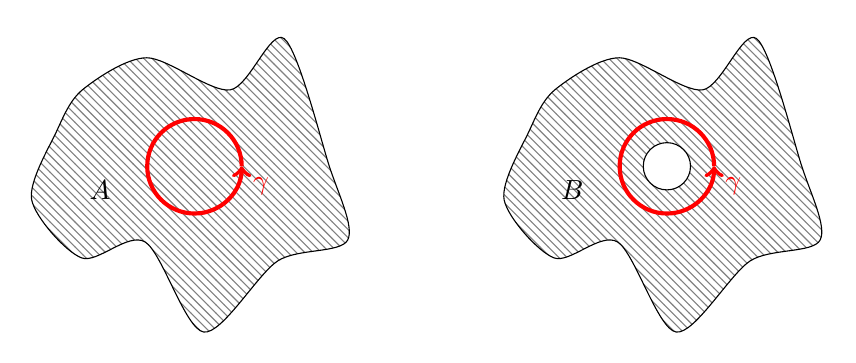
\begin{tikzpicture}[scale=1.5,
      set/.style={pattern=north west lines, pattern color=gray,fill opacity=.3},
      curve/.style={->,color=red,line width=1.5pt}
      ]
      \begin{scope}
        \pgfmathsetseed{3}
        \draw[set] plot [smooth cycle, samples=12,domain={1:8}] (\x*360/8+5*rnd:0.5cm+1cm*rnd) node at (0,0) {};
        \node at (-.8,-.2) {$A$};
        \draw[curve] (.4,0) arc (0:360:.4) node[anchor=north west] {$\gamma$};
      \end{scope}

      \begin{scope}[shift={(4,0)}]
        \pgfmathsetseed{3}
        \draw[set] plot [smooth cycle, samples=12,domain={1:8}] (\x*360/8+5*rnd:0.5cm+1cm*rnd) node at (0,0) {};
        \node at (-.8,-.2) {$B$};
        \draw[fill=white] (0,0) circle (.2);
        \draw[curve] (.4,0) arc (0:360:.4) node[anchor=north west] {$\gamma$};
      \end{scope}
    \end{tikzpicture}
  \end{center}
  Während $A$ einfach zusammenhängend ist, kann man bei $B$ die eingezeichnete Kurve $\gamma$ nicht auf einen Punkt zusammen ziehen, da sie das ``Loch'' innerhalb von $B$ umschließt. 
  Natürlich gibt es auch in $B$ Kurven, die auf einen Punkt zusammenziehbar sind.
\end{remark}

\end{document}
